\chapter{Software Architecture}

Architecture is the fundamental organization of a software system, embodied in its components, their relationships to each other and to the environment, and the principles guiding its design. The software architecture affects \emph{performance, usability, security, reliability, maintainability}, and so on.

Architecture is made up of \textbf{components}, where components implement a coherent set of \textbf{features} (services that may be used by other components). Here's an example of component usage:

\begin{figure} [H]
    \centering
    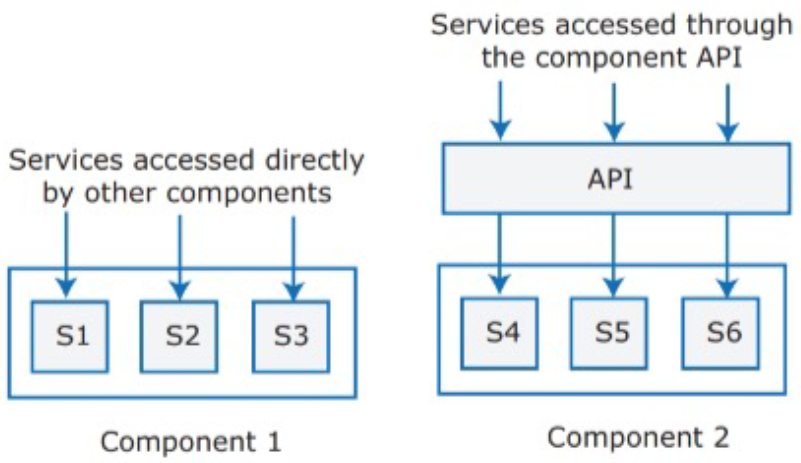
\includegraphics[width=0.7\textwidth]{images/SoftwareArchitecture/componentAPI.png}
    \caption{API to call component services}
    \label{fig:componentAPI}
\end{figure} 

In all cases where the software is large, developers will need to develop \textbf{APIs} (Application Programming Interfaces) to allow communication between components that might even be implemented with different technologies. \\

When we design our software, we need to take into account different aspects. These are some issues that are usually addressed:

\begin{itemize}
    \item \textbf{Non-functional product characteristics}: Non-functional product characteristics such as security and performance affect all users. If you get these wrong, your product is unlikely to be a commercial success. All these characteristics have a cost (e.g., availability, security, and so on).
    \item \textbf{Product lifetime}: If you anticipate a long product lifetime, you need to create regular product revisions. You therefore need an architecture that can evolve, so that it can be adapted to accommodate new features and technologies.
    \item \textbf{Software reuse}: You can save a lot of time and effort if you reuse large components from other products or open-source software. However, this constrains your architectural choices because you must fit your design around the software that is being reused.
    \item \textbf{Number of users}: If you are developing consumer software delivered over the internet, the number of users can change very quickly. This can lead to serious performance degradation unless you design your architecture so that your system can be quickly scaled up and down.
    \item \textbf{Software compatibility}: For some products, it is important to maintain compatibility with other software so that users can adopt your product and use data prepared using a different system. This may limit architectural choices, such as the database software that you can use.
\end{itemize}

\section{Non-functional Quality Attributes}

When we talk about \textbf{non-functional product characteristics}, we are defining a set of specifications that describe the system’s operational capabilities and constraints and attempt to improve its functionality. This is a list of the most popular ones:

\begin{itemize}
    \item \textbf{Responsiveness}: Does the system return results to users in a reasonable time? 
    \item \textbf{Reliability}: Do the system features behave as expected by both developers and users? 
    \item \textbf{Availability}: Can the system deliver its services when requested by users?
    \item \textbf{Security}: Does the system protect itself and users' data from unauthorized attacks and intrusions?
    \item \textbf{Usability}: Can system users access the features they need and use them quickly and without errors? 
    \item \textbf{Maintainability}: Can the system be readily updated and have new features added without undue costs?
    \item \textbf{Resilience}: Can the system continue to deliver user services in the event of partial feature failure or an external attack?
\end{itemize}

For each non-functional quality attribute we implement, we also need to test them. This increases the product cost. 
Usually, optimizing one non-functional attribute affects others (e.g., to achieve more security with longer keys, we may need to sacrifice some performance or usability).

The prototypes don't need to respect these characteristics because we want to quickly build a prototype. \\

\emph{Good practice} for maintainability is to decompose the system into small, self-contained parts and avoid shared data structures. Not having centralized data structures is a good practice because if one component needs to change the database organization, this does not affect the other components. The system can also continue to provide partial service in the event of a database failure.

\begin{figure} [H]
    \centering
    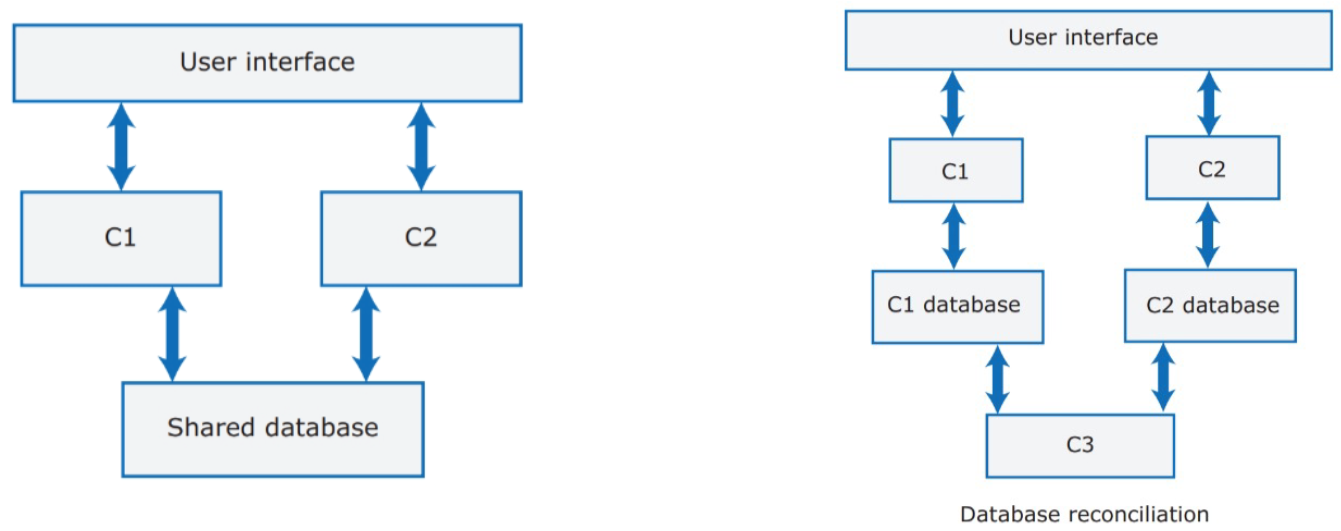
\includegraphics[width=0.9\textwidth]{images/SoftwareArchitecture/shattedDB.png}
    \caption{Database partitioning}
    \label{fig:shattedDB}
\end{figure} 

The cost of this practice is \emph{eventual consistency}: if component C1 makes a change (see Figure \ref{fig:shattedDB}), sooner or later that change must be reported to the C3 database. This is an additional cost. This also applies in the case of availability: if you want more availability, you can deploy multiple databases, but this requires synchronizing multiple databases. When something goes wrong in a distributed system, it's hard to roll back transactions. That's why we usually give up on consistency in order to achieve availability.

\newpage

\section{System Decomposition}

As we already said, a \emph{service} is a coherent unit of functionality, a \emph{component} is a software unit offering one or more services, and a \emph{module} is a set of components.

\begin{figure} [H]
    \centering
    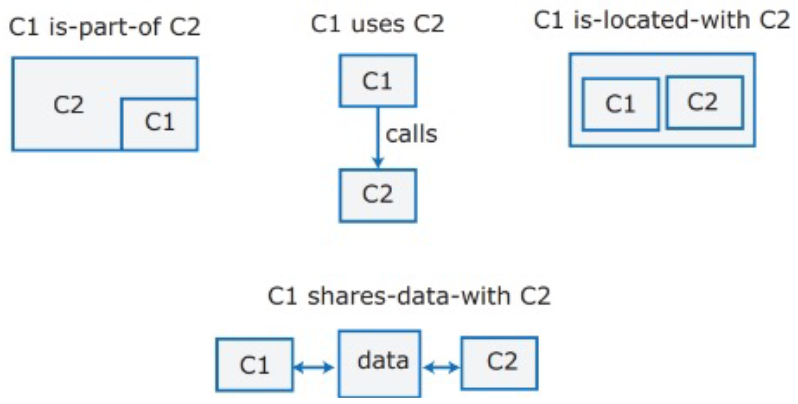
\includegraphics[width=0.7\textwidth]{images/SoftwareArchitecture/componentrelationship.png}
    \caption{Example of component relationships}
    \label{fig:componentrelationship}
\end{figure} 

As the number of components increases, the number of relationships tends to increase at a faster rate. Therefore, we should \textbf{decompose} as much as needed. The reason we want to decompose is to have simpler parts that can be maintained separately. In order to decompose a system, one good idea is \emph{separation of concerns}, as we will see with microservices that implement one business feature. We also want to have \emph{stable interfaces}, unless this is really necessary. The dogma of \emph{implement once} contrasts with the idea of independent teams that work with independent systems, but there aren't fixed rules; we always need to find trade-offs.

\begin{figure} [H]
    \centering
    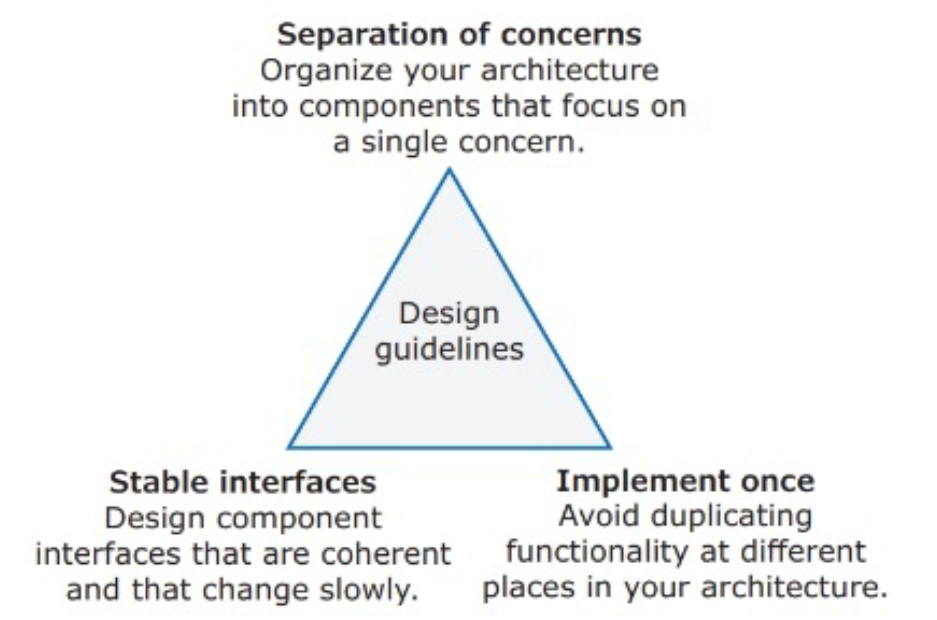
\includegraphics[width=0.7\textwidth]{images/SoftwareArchitecture/designguidelines.png}
    \caption{Design guidelines to control complexity}
    \label{fig:designguidelines}
\end{figure}

\newpage

Another aspect of system decomposition is having a \textbf{layered architecture}. Each layer is an area of concern and is considered separately from other layers. Within each layer, the components are independent and do not overlap in functionality. The architectural model is a high-level model that doesn't include implementation information. Software architects usually customize \emph{generic layers} by adding or removing layers until the architecture achieves a good form for its goals.

\begin{figure} [H]
    \centering
    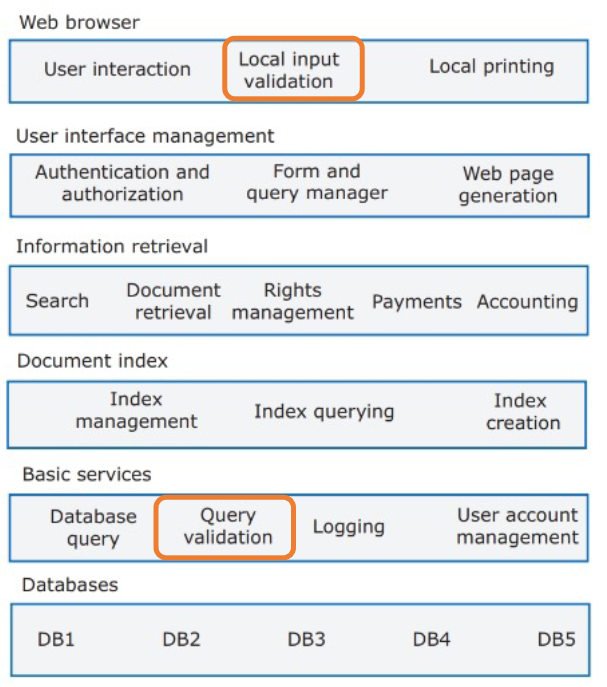
\includegraphics[width=0.7\textwidth]{images/SoftwareArchitecture/layaredarchitecture.png}
    \caption{Example of a layered architecture}
    \label{fig:layaredarchitecture}
\end{figure}

There are some systemic concerns that affect the whole system, so every layer must take them into account. \textbf{Cross-cutting concerns} (such as \emph{security, performance, reliability, validation}, and so on) add interactions between the layers. In the example shown in Figure \ref{fig:layaredarchitecture}, we can see that validation is considered in multiple layers. \\

On one hand, when we design architecture, we don't want to discuss implementation (because we don't want to limit the design with implementation details), but at the same time we need to consider possible implementations to understand how to design the architecture (e.g., the choice of using a relational database affects components at higher layers).

\section{Distribution Architecture}

The \textbf{distribution architecture} defines servers and the allocation of components to servers, specifying where the software will be deployed and run during production. \\

The most common type is the \textbf{client-server architecture}, which is suited for applications in which clients access a shared database and perform business logic operations on that data. Clients interact with \emph{load balancers} in the system, which are deployed on a cluster of servers.

\begin{figure} [H]
    \centering
    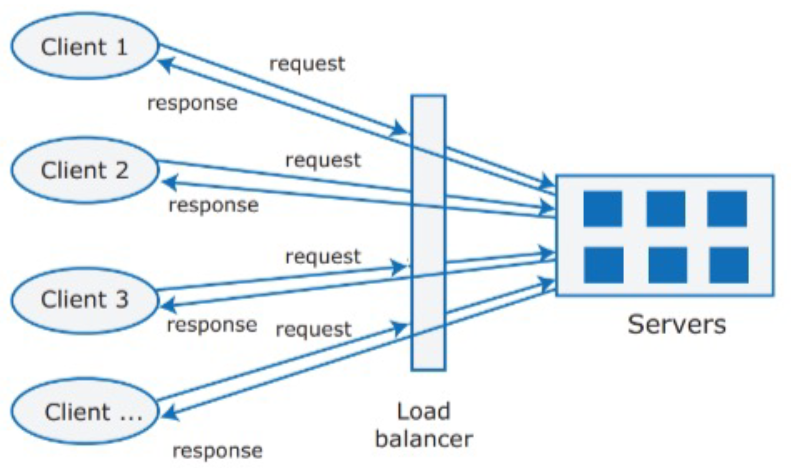
\includegraphics[width=0.7\textwidth]{images/SoftwareArchitecture/clientserverarchitecture.png}
    \caption{Example of a client-server architecture}
    \label{fig:clientserverarchitecture}
\end{figure}

\begin{wrapfigure}{r}{0.5\textwidth}
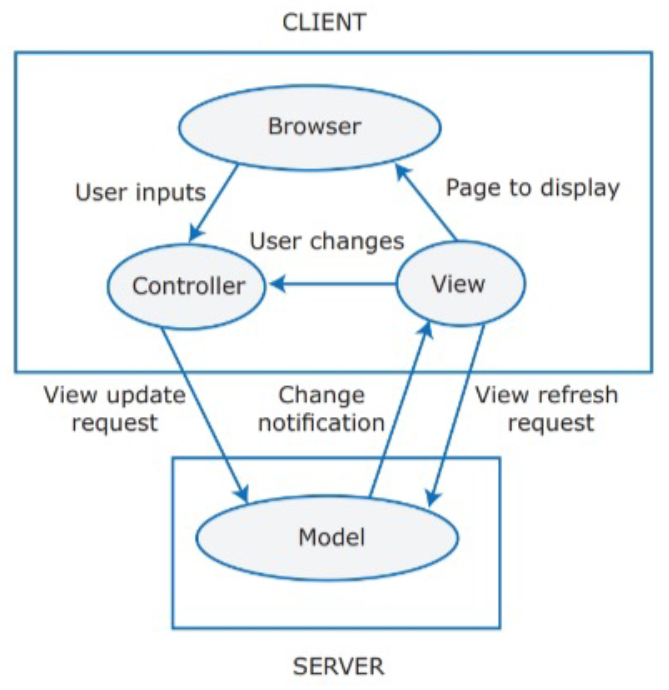
\includegraphics[width=0.45\textwidth]{images/SoftwareArchitecture/MVC.png}
    \caption{Model-View-Controller}
    \label{fig:MVC}
\end{wrapfigure}

\vspace{0.5cm}
\textbf{Model-View-Controller} is a widely used \emph{pattern}. This pattern helps to structure the code by dividing it into the \textit{Model part}, the \textit{View part}, and the \textit{Controller part}. In many cases, this also helps to understand how to implement the communications between the parts, which affects the simplicity and efficiency of the architecture (in many cases, the communication is implemented with HTTP + JSON). 

The pattern shown in Figure \ref{fig:MVC} is able to separate the logic of data presentation from business logic. This pattern is positioned at the logical or business level and is presented in a multi-tier architecture.

\newpage

\begin{figure} [H]
    \centering
    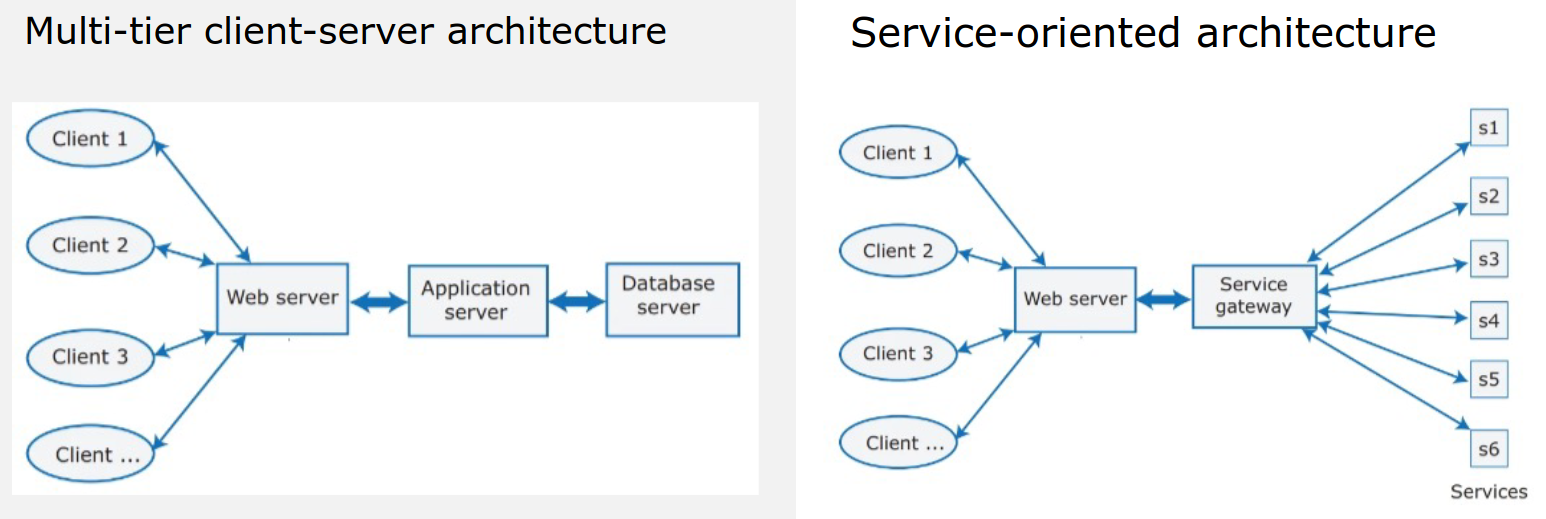
\includegraphics[width=1\textwidth]{images/SoftwareArchitecture/architectures.png}
    \caption{Common types of client-server architecture}
    \label{fig:architectures}
\end{figure}

Client-server architectures can be implemented in different ways (as shown in Figure \ref{fig:architectures}). The \textit{Service-oriented architecture} is slightly different: it has a Service gateway which splits the service requests to the appropriate service.
\newline\noindent
The choice of distribution architecture depends on several factors:
\begin{itemize}
    \item \textbf{Data type and data updates}: If you are mostly using structured data that may be updated by different system features, it is usually best to have a single shared database that provides locking and transaction management. If data is distributed across services, you need a way to keep it consistent, and this adds overhead to your system.
    \item \textbf{The system execution platform}: If you plan to run your system on the cloud with users accessing it over the Internet, it is usually best to implement it as a service-oriented architecture because scaling the system is simpler. If your product is a business system that runs on local servers, a multi-tier architecture may be more appropriate.
    \item \textbf{Change frequency}: If you anticipate that system components will be regularly changed or replaced, then isolating these components (inside containers) as separate services simplifies those changes.
\end{itemize}

\section{Technology Choices}

There are several ``relevant'' technology choices. These are considered relevant because changes in product design will reflect on these technologies, resulting in increased complexity and costs required to modify them during development.

\newpage
\noindent
This is a list of some relevant technologies:
\begin{itemize}
    \item \textbf{Database}: You should use either a \textit{relational SQL database} (where data is organized into structured tables, particularly suitable when transaction management is needed and data structures are predictable and simple) or an \textit{unstructured NoSQL database} (where data has a more flexible, user-defined organization. This option is more efficient for data analysis, and data can be organized hierarchically. It also supports efficient concurrent processing of 'big data').
    \item \textbf{Delivery Platform}: This refers to the platform where the product will ultimately run. Delivery can be web-based or mobile, but each platform presents its own challenges (e.g., mobile device issues include intermittent connectivity, processor power, power management, reduced screen size, and on-screen keyboard). It's advisable to decide on the platform early in order to begin the development phase as soon as possible.
    \item \textbf{Server}: Will the product run in a public cloud, or will it use in-house servers? Most consumer products utilize a set of microservices, which are containerized and deployed in the cloud (with their Service-Oriented Architecture, SOA). In contrast, business products are more concerned with cloud security issues (e.g., where and how client data will be stored). Once it's decided that the product will be launched in the cloud, the next decision is to choose a provider (note that it can be challenging to migrate a product across cloud providers due to vendor lock-in).
    \item \textbf{Open Source}: Are there suitable open-source components that could be incorporated into the product? Are these open-source components secure enough?
    \item \textbf{Development Tools}: Development technologies (e.g., mobile development toolkits, web application frameworks) influence the architecture of your product. The development technology that developers are familiar with may indirectly affect the architecture of the product.
\end{itemize}

\section{Enterprise Application Integration}

\textbf{Enterprise applications} are large software systems typically designed to operate in a corporate environment, such as business or government. These applications are extensive systems where users can typically only see the front-end, while a lot of backend functionality (made up of multiple services) supports it. The various heterogeneous services can be classified as \emph{sources} (services that only make requests), \emph{sinks} (services that only respond to requests), or a mix of both categories. These services communicate using various \emph{heterogeneous data types} (with different representations, even for analogous data), and this information can be shared with \emph{different organizations} over the \emph{network}. This complexity makes enterprise applications distributed multi-service applications whose services must work together and be suitably integrated.

The architectural question is how to integrate all of this in a coherent, extensible, and maintainable way. There is a need to manage these complexities, and one approach is to use \textbf{patterns}. A pattern is a high-level abstraction of accepted, reusable solutions for recurring problems. Patterns are defined in terms of problem statements (what problem the pattern solves), context (there may be different patterns for the same problem), forces (why you should consider using a pattern for the problem), and solutions (how to apply the pattern to solve the problem). The idea of patterns is to avoid reinventing the wheel and instead use established patterns. \textbf{Enterprise Application Integration} (EAI) is a reusable abstraction of proven solutions to well-known problems that arise while integrating the software components and services forming enterprise applications. 

\subsection{Patterns}

These patterns were studied more than 20 years ago. Among all the patterns, the most commonly used are \textbf{messaging patterns}, as shown in Figure \ref{fig:EIPpatterns}.

\begin{figure} [H]
    \centering
    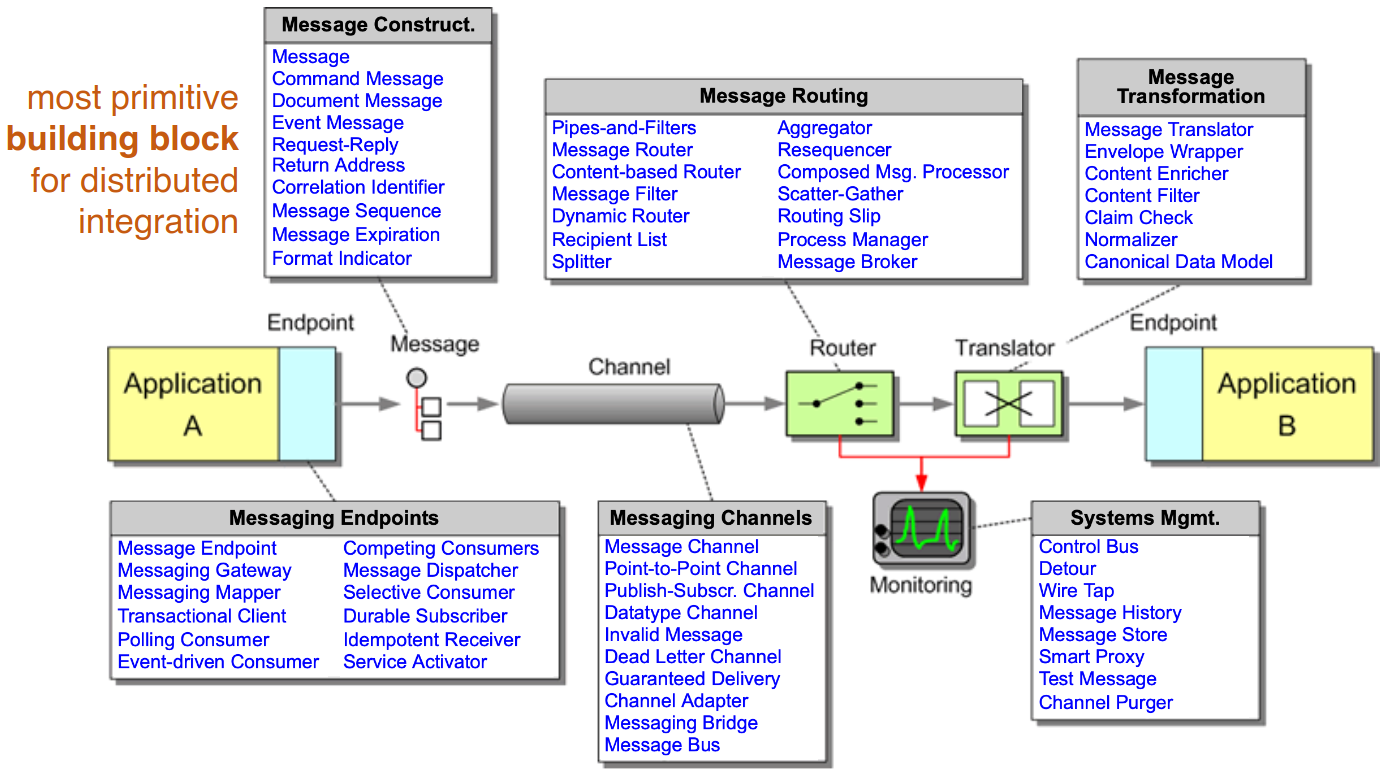
\includegraphics[width=1\textwidth]{images/SoftwareArchitecture/EIPpatterns.png}
    \caption[Caption for EAI messaging patterns]{Messaging Patterns\protect\footnotemark}
    \label{fig:EIPpatterns}
\end{figure}
\footnotetext{\url{https://www.enterpriseintegrationpatterns.com/patterns/messaging/}}

A message is a discrete piece of data sent from one service to another. Typically, messages are structured into a \textit{header} (metadata) and a \textit{body} (payload). Concrete examples of messages include \emph{document messages} (pure data), \emph{event messages} (notifications of events), and \emph{command messages} (commands sent to perform actions).

\begin{figure} [H]
    \centering
    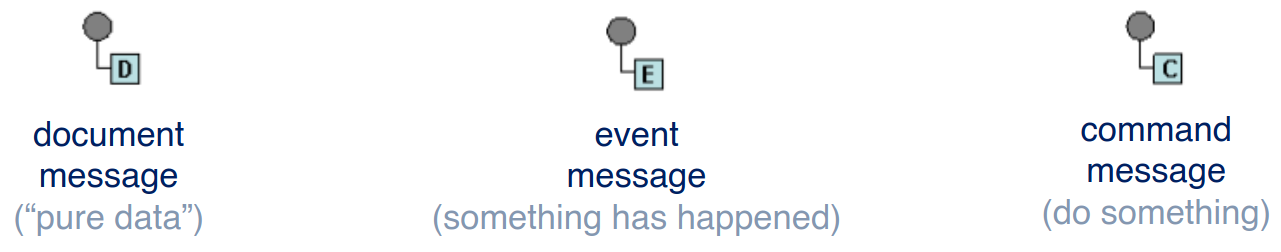
\includegraphics[width=1\textwidth]{images/SoftwareArchitecture/AEImessages.png}
    \caption{Example of concrete messages}
    \label{fig:AEImessages}
\end{figure}

The exchange of messages means that the services are not tightly connected but can communicate through messages. Message-based communication enables \emph{loose coupling}, and it is realized through \textbf{channels}: abstractions for components sending messages from a source to a destination (implemented in various ways, such as RPC, HTTP, TCP, and so on). Channels are \emph{one-way}, allowing communications to be natively asynchronous. Synchronous (request/response) communications use two channels. Application services are typically independent of the messaging systems; thus, \textbf{adapters} are used to enable application-specific data to be sent to channels. \textbf{Message endpoints} allow application services to send and receive messages to and from channels. There are different types of channels: the one shown in Figure \ref{fig:AEIsimpleintegration} is a \emph{point-to-point} channel (which ensures that only one receiver will receive a particular message), whereas another type is the \emph{publish-subscribe} channel (where the publisher delivers a copy of incoming messages to each subscriber).

\begin{figure} [H]
    \centering
    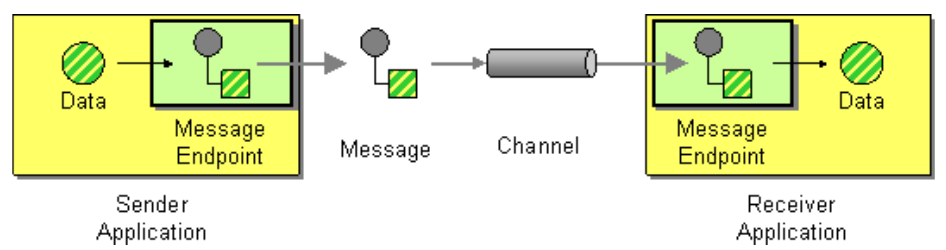
\includegraphics[width=1\textwidth]{images/SoftwareArchitecture/AEIsimpleintegration.png}
    \caption{Simple integration of message-based communication}
    \label{fig:AEIsimpleintegration}
\end{figure}

This implementation alone is not sufficient: what happens if the receiving service expects a different data format? A \textbf{message translator} allows the message to be adapted to suit the receiving services, but additional steps may still be necessary (e.g., how to route messages to different or multiple endpoints, how to split messages, and how to aggregate messages).

\newpage

\subsection{Pipes and Filters}

The \textbf{pipes and filters architectural style} (along with other EIPs) enables structuring the more complex integrations required by enterprise applications. Messages pass through multiple processing steps/components (the filters), while components send messages down the channels (pipes) to which they are connected. The idea is that messages flow through the pipes, and as they reach a filter, they may be transformed before reaching the sink (the target of the message). \\

One of the most common examples in the field of EAI is the \emph{Loan and Broker design}: the \emph{loan company} sends a request, the \emph{Credit Bureau} validates the request, the \emph{Rule Base} decides which office should process the request, and then the \emph{Banks} will be notified to accept or reject the loan. All the responses will be aggregated and sent back to the loan company. The shaded area in the Loan Broker example represents the Loan service.

\begin{figure} [H]
    \centering
    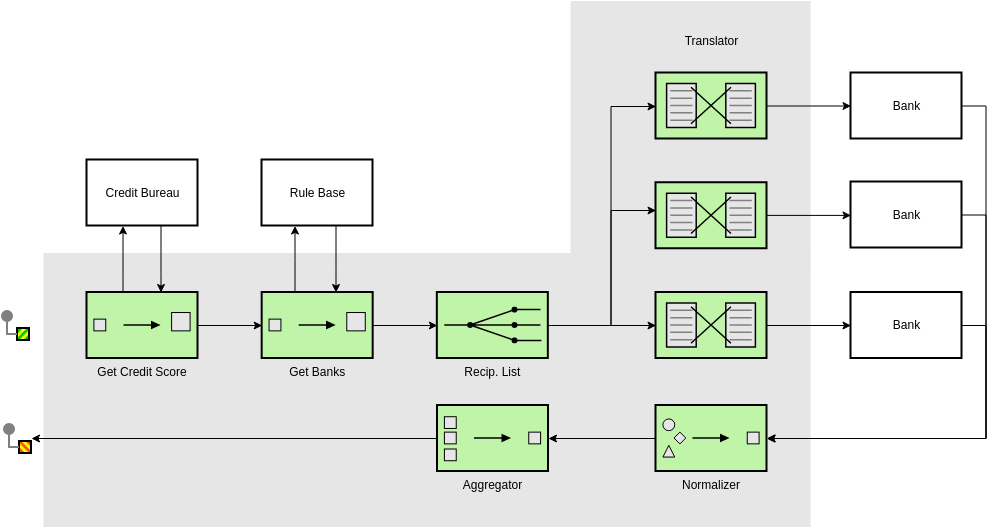
\includegraphics[width=1\textwidth]{images/SoftwareArchitecture/EAIloanbroken.png}
    \caption{Loan Broker Design}
    \label{fig:EAIloanbroken}
\end{figure}

This is a list of additional patterns used that haven't been described until now:

\begin{itemize}
    \item \textbf{Content Enricher}: This pattern uses information within the incoming message (e.g., key fields) to retrieve data from an external source. In the example shown in Figure \ref{fig:EAIloanbroken}, the calls \emph{Get Credit Score} and \emph{Get Banks} are examples of content enrichment. Retrieved data is appended to the message. Original information may either be retained or discarded.
    \item \textbf{Routers}: There are mainly two categories for message routing: \emph{content-based routers} route messages based on message type (in headers) or message content (in the body), while \emph{context-based routers} route based on contextual information retrieved from a central configuration location.
    
    In general, a message router connects to multiple channels and contains the logic to decide which channel it should send to.

    \begin{figure} [H]
        \centering
        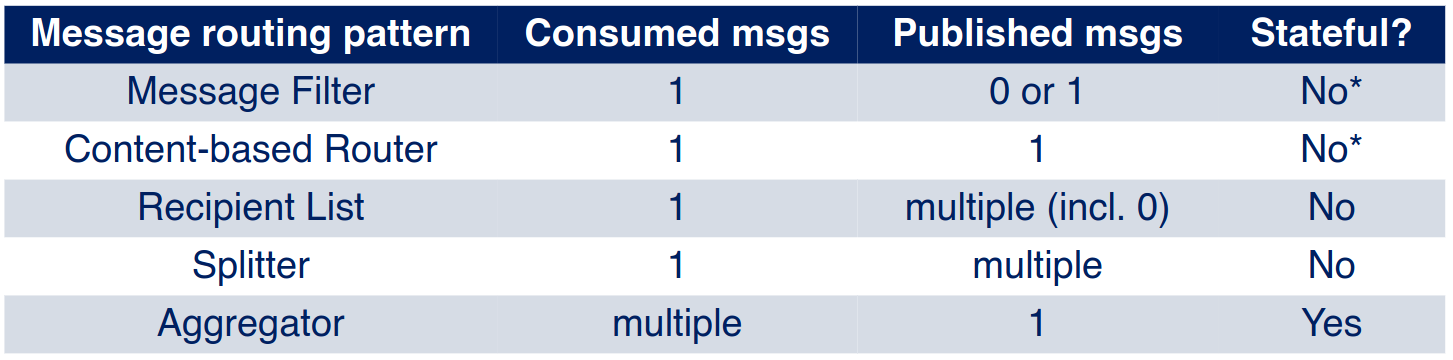
\includegraphics[width=1\textwidth]{images/SoftwareArchitecture/messageRoutingpattern.png}
        \caption{Message routing patterns}
        \label{fig:messageRoutingpattern}
    \end{figure}
    
    A \textbf{recipient list} inspects an incoming message, determines the list of desired recipients, and forwards the message to all channels associated with the recipients in the list. A \textbf{content-based router} enables routing each message to the correct recipient based on the message content.
    \item \textbf{Normalizer}: This pattern enables translating messages to match a common data format. This is usually realized as a composition of multiple patterns: it is possible to combine several patterns to create \emph{composite patterns} (as is the case with the normalizer).
    
    \begin{figure} [H]
        \centering
        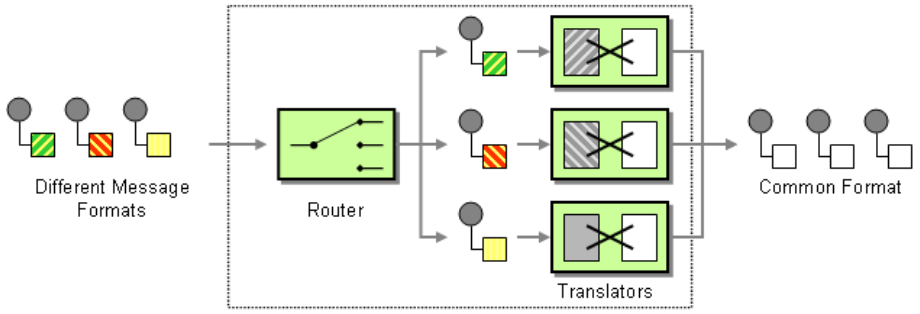
\includegraphics[width=0.9\textwidth]{images/SoftwareArchitecture/normalizer.png}
        \caption{Normalizer schema}
        \label{fig:normalizer}
    \end{figure}

    \item \textbf{Aggregator}: A (\emph{stateful}) aggregator collects and stores individual messages until a complete set of related messages has been received (see Figure \ref{fig:messageRoutingpattern} for reference). This is usually utilized when some integration steps may occur in parallel: independent processes can be executed in parallel, and the results of these processes can be aggregated to inform subsequent decisions on how to proceed.
\end{itemize}




